% !TeX spellcheck = en_GB
\documentclass[../summary.tex]{subfiles}
\usepackage{graphicx}

\begin{document}

\section{Migration}

\subsection{Study guide}
For this chapter you will need to have a good understanding of the following concepts and definitions:
\begin{itemize}
	\item Definition of migrant by UN standards, migration corridors, refugees, asylum-seekers, indentured workers and IDPs, slow- and fast-onset events, trapped populations
	\item Concepts of stock versus flow, ``Out of Africa'' thesis, age of discovery, triangular trade system and its consequences, labour immigration, push-pull model, migration transition model, the ``maximalist'' or ``Neo-Malthusian'' view and the migration hump theory.
\end{itemize}

\subsection{Migrant $\neq$ Migrant}
\subsubsection{what are migrants and how are they counted}
Firstly the definition of a migrant is given by the UN Migration agency and is defined as:
\begin{quote}
	\textbf{Any person who is moving or has moved across an international border or within a State away from his/her habitual place of residence, regardless of:}
	\begin{enumerate}
		\item \textbf{Legal status}
		\item \textbf{Whether the movement is voluntary or involuntary}
		\item \textbf{The cause of the movement}
		\item \textbf{Length of stay}
	\end{enumerate}
\end{quote}
This definition of migration is a sub-category in a more general concept of \textbf{global mobility}, which also includes circulation. A simple question with no simple answer is; how many migrants are there in the world? To answer this, two new terms are introduced, stock and flow statistics

\begin{description}
	\item[Stock statistics] count the number of people with some characteristic at a given point in time in some geographic area. An example of this is the amount of migrants in Belgium on the $\mathrm{1^{st}}$ of January, 2020.
	\item[Flow statistics] count events over a period of time. An example of this is the amount of immigrants that entered Belgium throughout 2020.
\end{description}
The distinction between these two terms is crucial, since it is possible for a country to have a very low number of immigrants entering in a given year, but still have a very high number of migrants living in that country in that same year (or the other way around).

\subsubsection{Migrant corridors}
Around to \textbf{3\% of the population is a migrant} according to the definition, and that percentage has been growing slightly. Although this might be due to ongoing migration transitions. Experts point out that \textbf{registration of migrants has improved}. Because of this there are \textbf{no indications that there has been a dramatic rise of migration} in recent years.
\\\\
Available data shows an estimation of origin and destination of migration. With this information \textbf{migration corridors} can be estimated. The size of a corridor between country A and B is defined as the number of people born in country A who are residing in country B at the time of the estimate. These migration corridors provide a snapshot of migration patterns and movements that form significant foreign-born populations in specific destinations.

\subsubsection{Refugees and asylum-seekers}
Although media focuses on refugees, this only represents 10\% of the worldwide stock of international migrants. For better understanding three terms have to be defined:
\begin{description}
	\item[Refugee] is a person ``owing the well-founded fear of being persecuted for reasons of race, religion, nationality, membership of a particular social group or political opinion, is outside the country of (their) nationality and is unable or, owing to such fear, is unwilling to avail (themself) of the protection of that country'', which is defined in international law by the 1951 Refugee Convention.
	\item[Asylum seeker] is someone who intends to seek or is awaiting a decision on their request for international protection. In some countries, it is used as a legal term for a person who has applied for refugee status and has not yet received a final decision on their claim .
	\item[Internally displaced people (IDPs)] have been forced to flee their homes by conflict, violence, persecution or disasters, however, unlike refugees, they remain within their own country.
\end{description}
The largest proportion of refugees and asylum-seekers are hosted in developing countries, typically in neighbouring countries.


\subsection{Major migration flows in history}
\subsubsection{Acceleration of migration before early modern period}
Migration is a hot topic lately, but has been going on for thousands of years. As homo sapiens originated from Africa they would have had to spread all over the world, this is called the \textbf{``Out of Africa''} thesis. In the middle ages, migration played a crucial role in development of the different societies. Due to advancements in transportation technologies - like navigation and sailing - migration has increased even more.

\subsubsection{Acceleration of migration in the early modern period}
Due to the technological advancements, colonisers migrated out of Europe, thereby starting the age of discovery. Using armed forces to colonise regions like Africa and Asia and later America. This ended in mass extermination of indigenous peoples where most died by diseases brought in by the Europeans. After establishing the colonies, the famous \textbf{triangular trade system} was set up, which was a major forced migration flow.
\\\\
Goods like textiles and guns where shipped from Europe and traded for slaves in West-Africa. Then these slaves would be shipped to America where they would be sold. Lastly the money would be used to buy products in America and ship them back to Europe. Not only was there \textbf{mass forced migration} but also \textbf{extreme dehumanising of non-European people}. This fuelled a racist ideology.
\newpage
\subsubsection{Slavery}
As seen in figure \ref{fig:slaves-captive}, the number of slaves imported increased rapidly until the trade triangle was demolished in 1815. Although there was no more importation of slaves, slavery still persisted. In fact, in 1865 the amount of slaves in America doubled from 3 to 6 million. Finally slavery was abolished at the end of the American Civil War.

\begin{figure}[h]
	\centering
	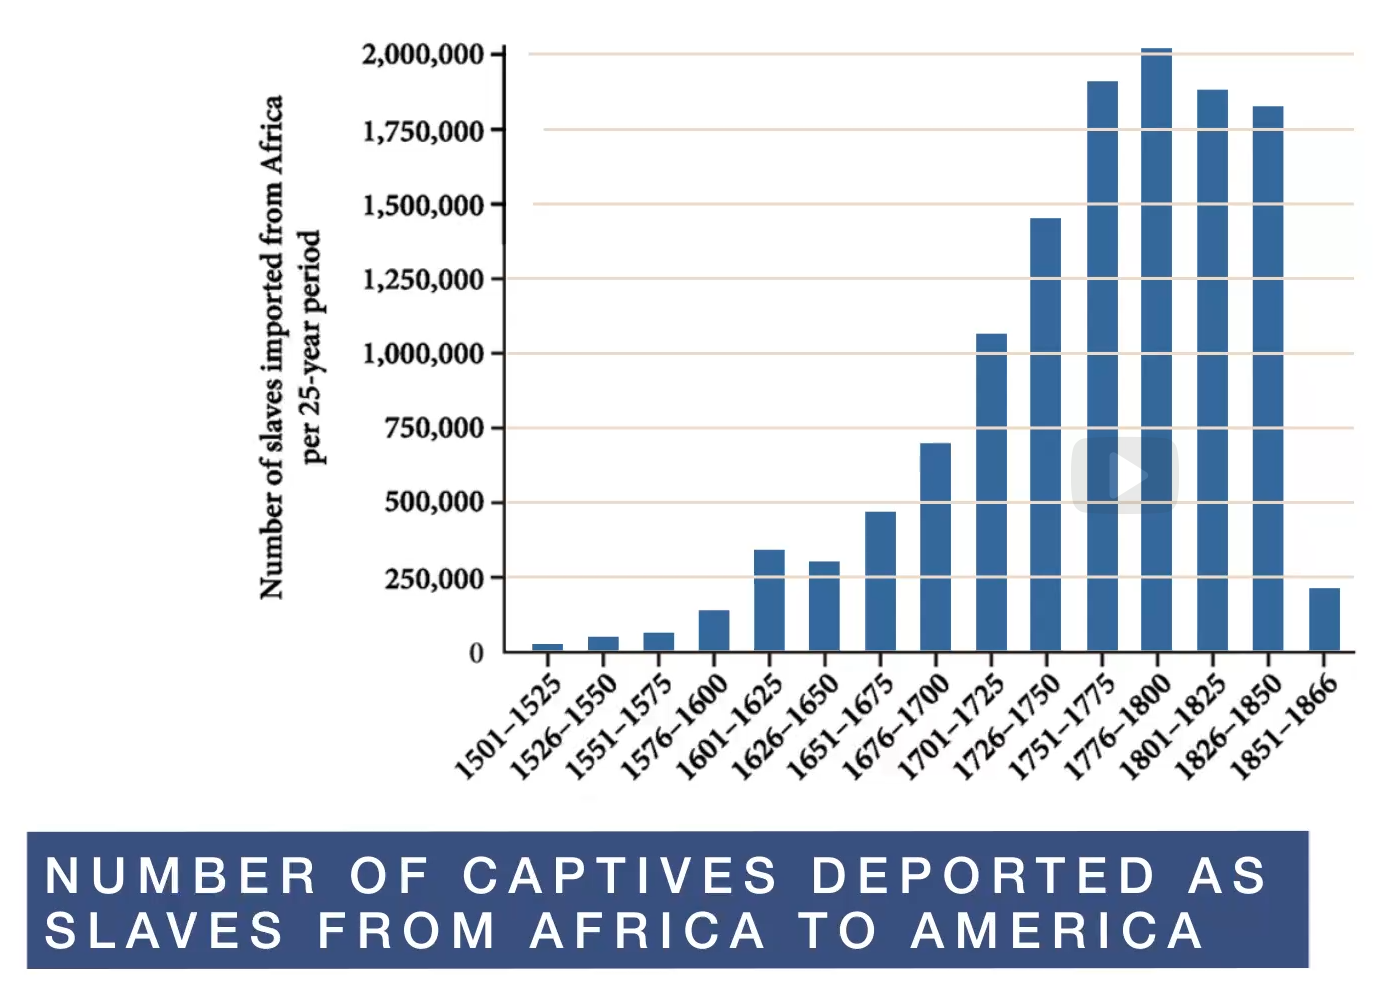
\includegraphics[width=0.7\linewidth]{../images/7-slaves-captive}
	\caption{Number of slaves held captive in America}
	\label{fig:slaves-captive}
\end{figure}

\subsubsection{Indentured workers}
In the second half of the $\mathrm{19^{th}}$ century a new system was invented, the so-called \textbf{indentured workers}. Low-paid workers were recruited from the Indian subcontinent and transported (sometimes by force) to America. It is important to note that these workers where not seen as property of the plantation owners. Between 12 and 37 million workers where shipped within this system and the consequences of this migration flow are still visible today.

\subsubsection{Era of industrialisation}
Due to the population growth and economic modernisation producing clothes, food and other provisions became more efficient. Because of the sudden growth in population and decrease in needed workers, the amount of unemployed people rose. This stimulated two large streams of migration. Firstly people massively moved from rural areas to urban areas to find employment in the developing industry. And secondly a major group immigrated out of Europe to other parts of the world like Australia and America.
\\\\
Between 1820 and 1987 around 54 million people moved to America, important origin countries include the UK, Ireland, Italy, Spain. This played a key role for the development of the America's economy, culture and industry.
\newpage

\subsubsection{World Wars}
The second World War generated the largest flow of refugees in Europe so far. The inter-war period was a period of mounting hostility against migration and immigrants. In the past migration policies where focused on trying to prevent people from leaving the country, because too much immigration would undermine the wealth of the country of origin. Since the first World War, migration policies have been altered to keep immigrants out. This is why after the first World War passports where introduced in multiple governments to prevent foreigners entering the country. Such passport requirement for migrants have since then become the rule across the globe.

\subsection{Migration Flows}
A very large amount of migration flows can be classified as labour migration, i.e, people moving to places where they hope to find a job instead of being unemployed, or with a higher salary and better working conditions than before. Nevertheless, migrant workers typically end up in the lower-paid and less-safe segments of the labour market in the country of destination (which may still be beneficial compared to the situation in the country of origin).

\subsubsection{Push-pull model}
The \textbf{push-pull model} is a model that is often used to explain migration. The bad conditions of the origin country are pushing people away while the good conditions in other country's are attracting them. Migration scientist no longer use this model because it does not accurately explain migration, leading expert Ronald Skeldon even calls this model ``a platitude at best''. Three points are made to prove that the model is not only a platitude but may also be misleading.
\begin{enumerate}
	\item This model would predict that the poorest people in the poorest countries will be the most likely to migrate. This prediction is wrong because these people don't have the money to migrate. Often it is the middle-class people in medium-developed countries that tend to migrate.
	\item Secondly, this model would predict that people in oppressive political regimes would have high migration rates, but in fact that is not the case since they are often not allowed to leave. Instability, insecurity and violent conflict even leads people to stay home to protect their property and family.
	\item Lastly, the model would predict that most people would go to the wealthiest and safest countries like Sweden or Norway, but that is not the case.
\end{enumerate}
As we can see the traditional \textbf{push-pull model is not sufficient}. We need to look at the factors that may hinder or facilitate migration from the area. Examples of this are:
\begin{itemize}
	\item Are origin and destination connected with trains, boats, etc.?
	\item Who can board available trains, planes, etc.?
	\item Who has the money to move?
	\item Who is allowed to move?
\end{itemize}
\newpage

\subsubsection{Framework of migration aspirations and capabilities}
\textbf{The framework of migration aspirations and capabilities} is a model that better predicts migration. History has shown that with improving socio-economic development, the aspirations to immigrate tend to first rise and then decline, forming an \textbf{inverted U-shape}.
\begin{figure}[h]
	\centering
	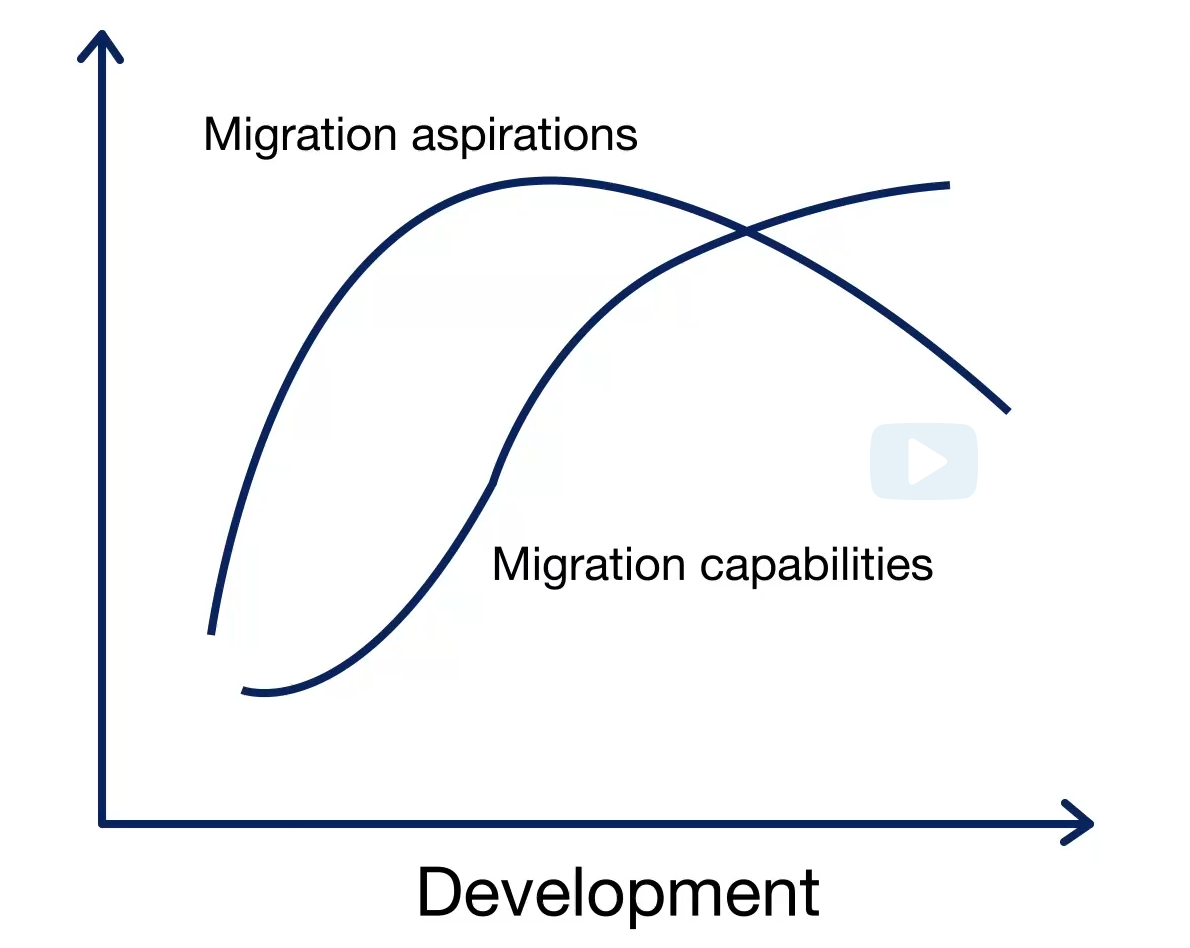
\includegraphics[width=0.6\linewidth]{../images/7-framework-capabilites}
	\caption{Migration and aspiration capabilities}
	\label{fig:framework-capabilites}
\end{figure}

An increase in development would lead to more people considering moving, but as development increases and living conditions get better, less people would want to leave. Whilst the migration capabilities initially rise when there is more development, the curve saturates as most people have reached a high enough wealth to be able to migrate.
\\\\
From the interplay between the migration aspirations and capabilities, actual out- and immigration rates emerge. This model is called the migration transition and is depicted in figure \ref{fig:migration-transition}. Because of this, highly developed countries often have high immigration and emigration rates.
\begin{figure}[h]
	\centering
	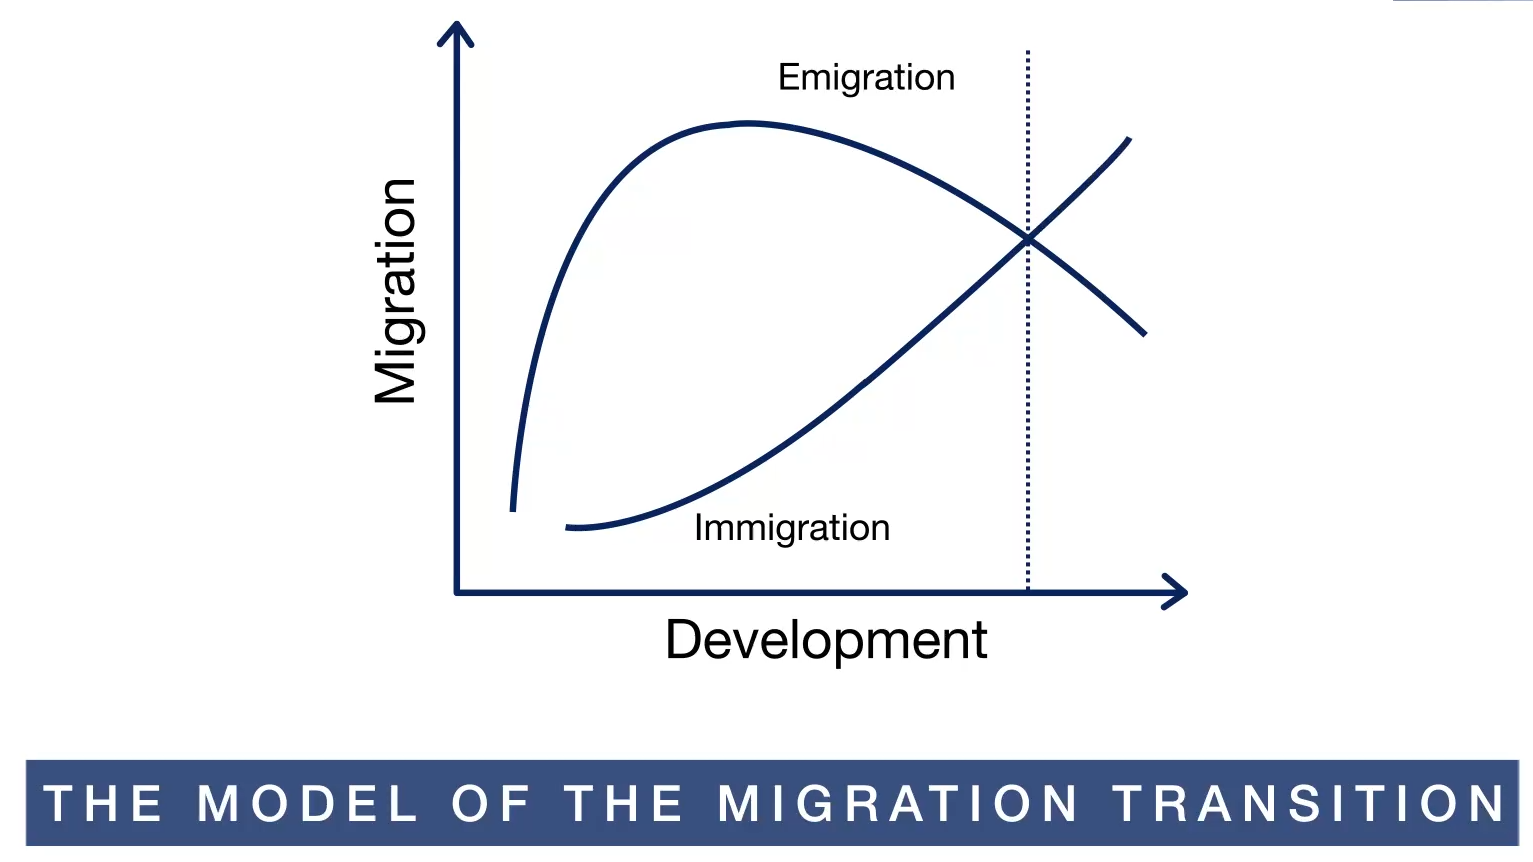
\includegraphics[width=0.7\linewidth]{../images/7-migration-transition}
	\caption{Migration transition}
	\label{fig:migration-transition}
\end{figure}


\subsection{Climate change and mobility}
Initially it was thought that climate change would lead to massive new migration flows. This rather simplistic view is now called ``the maximalist'' or ``Neo-Malthusian'' view. This view is based on the idea that climate change would cause droughts, floods, rising sea level, etc... causing people to be forced to move and thereby causing massive climate migration. Further research proved that this theory was wrong. There are several reasons for this:
\begin{enumerate}
	\item Migration is only one of the adaptive reactions as a result of climate change. Other examples are heightening dikes or using air-conditioning. Adaptive measure such as these often have a lower cost than migration.
	\item The theoretical ideas about migration underlying the original studies were to simplistic. The cultural and economical circumstances where not properly taken into account.
\end{enumerate}
More recent studies suggest that climate change may lead to more, less or an equivalent amount of migration. These three scenarios are depicted in figure \ref{fig:climate-change}.
\begin{figure}[h]
	\centering
	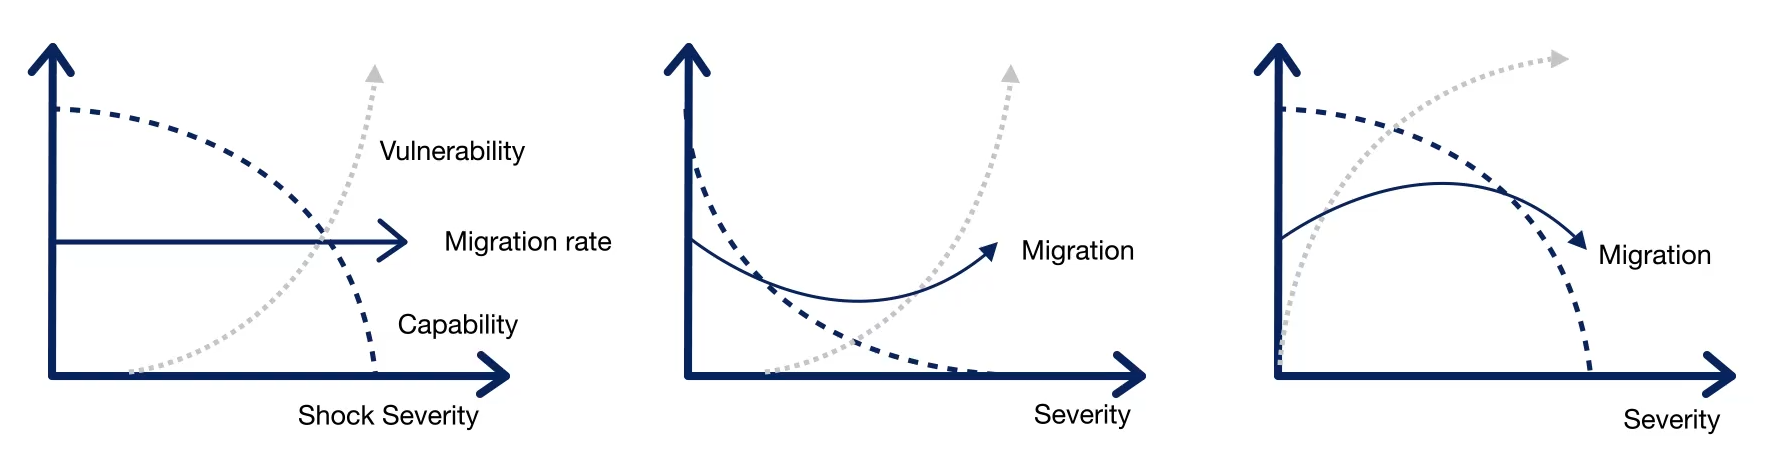
\includegraphics[width=0.7\linewidth]{../images/7-climate-change}
	\caption{Possible effects of climate change on immigration}
	\label{fig:climate-change}
\end{figure}
Predicting immigration due to climate change is not a simple task. When looking at different \textbf{modifying factors} that have an effect it can be concluded that they often affect the capability but also the vulnerability. For example, having a high income and a solid social network will help people to be less vulnerable to bad weather and therefore be more likely to stay. But on the other hand these resources have a positive effect on the capability to migrate. In all these types of cases \textbf{it is not clear if this will lead to higher or lower immigration}.

\subsubsection{Trapped populations}
Rather than being forced to leave, \textbf{households with low resources are often forced to stay}, even if they are highly vulnerable to extreme weather events. This has already caused many human casualties, such as during the heat-waves striking major cities in Asia in the spring of 2024.

\subsection{Migration policies}
As previously mentioned, initial migration policies were focused on preventing people from leaving the country and thus undermining the size, strength and wealth of a country. However after the First World War, more \textbf{restrictive migration policies} were introduced. This meant that the government was increasingly trying to monitor who was allowed in. This is the period where the passport requirement was introduced.
\\\\
After the Second World War, many European nation states started to develop \textbf{active labour immigration policies}, since an enlarged labour force was deemed needed to rebuild the national infrastructures and economies. Since there was also a very high number of refugees, the refugee convention, often called the \textbf{``Geneva Convention''} was signed.

\newpage

\subsubsection{Active labour immigration policies}
To rebuild national infrastructures and economies European countries competed against each other to attract more immigrants. This period came to an end with the international economic crisis. Europe then decided to sign the \textbf{Schengen Agreement}, which created a large international area \textbf{without internal border control}. As a result, European politics became more focused on \textbf{external border control}, and invested millions to keep migrants out. Still immigrations rates rose.

\subsubsection{Rise of immigration rates in Europe}
The scientific literature mentions \textbf{4 substitution methods} that help explain why the immigration rates of Europe keep on rising.
\begin{description}
	\item[Spatial subsitution] when sea routes A and B have been covered, routes C and D pop up. Migrants have always found new routes and it seems impossible to close all possible routes.
	\item[Categorical subsitution] When legal channel A has been blocked, people turn to channel B, or C, or D, these can be legal or illegal. An example of a legal channel is marriage migration, and an example of an illegal categorical substitution is overstaying student visa.
	\item[Temporal subsitution] For example when politicians announce that they will close a border, causing a ``now-or-never'' migration to happen.
	\item[Reverse flow subsitution] This happens when stricter migration policies lead to a bigger reduction of emigration than of immigration.
\end{description}
So, as a result of the four substitution mechanisms, migration policies aimed to close the border may have quite different results than expected.

\subsubsection{``Why boat refugees don't fly''}
Although plane tickets are 3 times cheaper than the dangerous boat rides that cross the Mediterranean sea, refugees often get stopped at the airline check-in and are rejected. This is due to the European directive that \textbf{every airline and boat-line that bring a person without the proper documents for entry, have to pay all the costs of returning that person back to their country of origin}. The only exception to this rule is refugees that come based on the Geneva Convention. By doing this the \textbf{European government has escaped responsibility }and transferred it to the staff at the check-in counter. So it is this directive that is the reason for so many refugees drowning in the Mediterranean sea.

\subsection{Cultural diversity and superdiversity}
Migration is contributing to the diversification of society. There is no such thing as a mono-cultural society and migration is just one of the many social mechanisms that creates cultural diversity, although this is unwanted by some people. Due to migration, more languages are spoken by people with a diverse cultural background in the same place. This concept is sometimes described as \textbf{superdiversity}. This has a quantitative dimension; namely that there are more people with a migrant background in many countries. And a qualitative dimension; migrants come from a diverse range of countries, from different regions, with diverse ethnic backgrounds, entering through a wide range of different channels.
\\\\
Research has shown that political parties who rally against immigration have been winning a lot of elections lately. This is because people grossly overestimate the proportion of people with a migrant background in their country. When confronted with the actual numbers, many people do not change their minds but rather claim that the statistics must be wrong. This is a kind of confirmation bias, that is the tendency of people to hear, remember and believe information in a way that confirms and supports prior beliefs. It is even found that media reinforces such sentiments and may strongly amplify anti-migration ideas.
\\\\
Studies have also shown that being in contact with refugees develops a more positive attitude towards migrants and migration.

\subsection{Migration hump theory}
In order to make immigration a win-win situation, we need to find ways to make migration safe and orderly. \textbf{Integration in the labour market} will be one of the key challenges.
\\\\
As countries of origin develop into high levels of economic development, emigration rates decline. Such findings have given rise to the migration hump theory. This is illustrated in figure \ref{fig:hump}.
\begin{figure}[h]
	\centering
	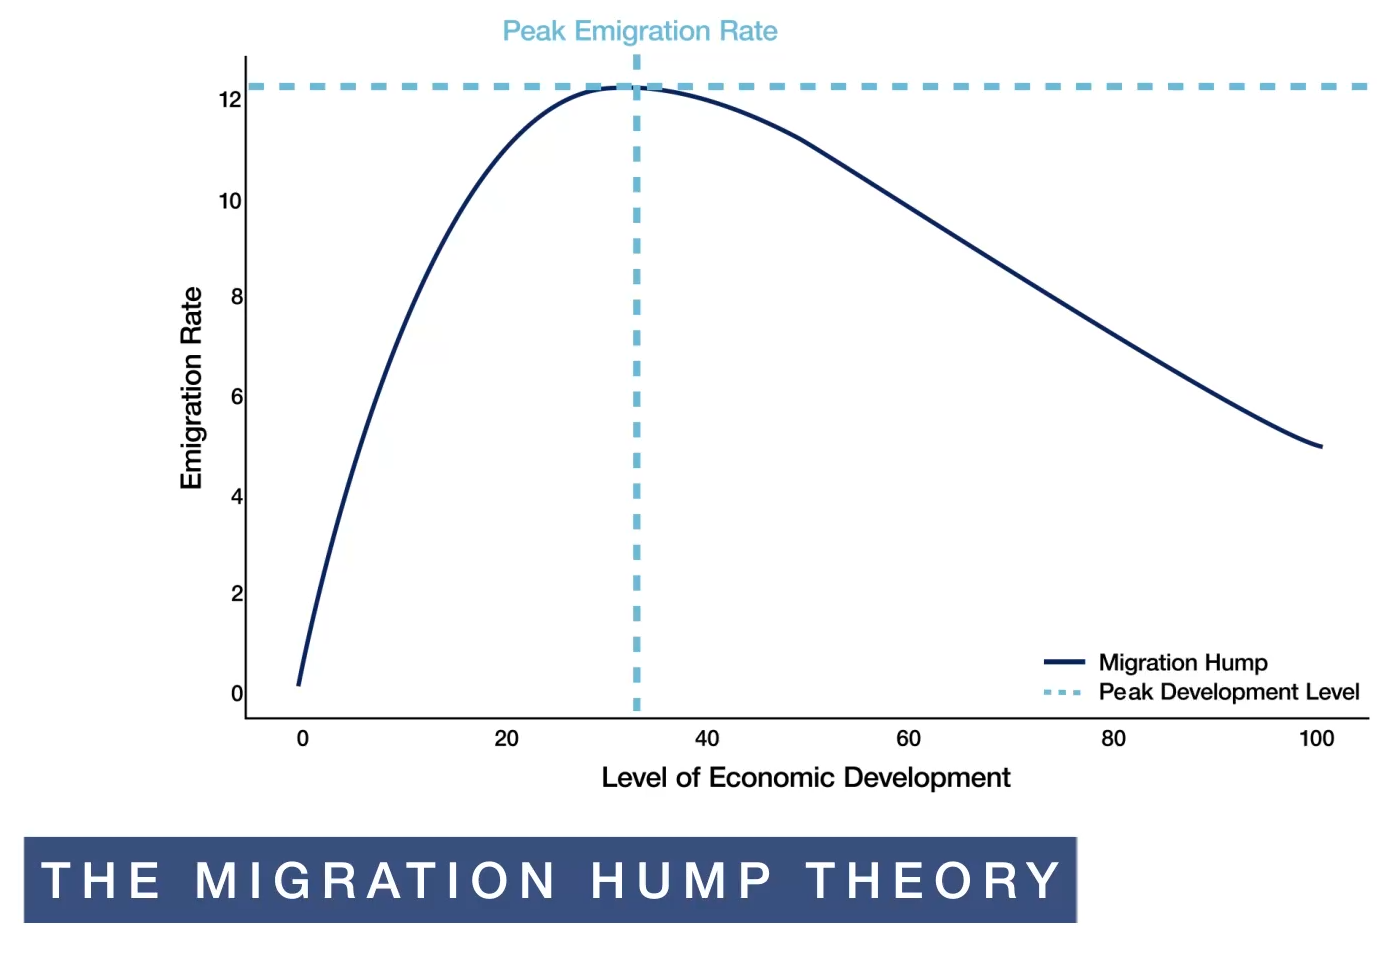
\includegraphics[width=0.7\linewidth]{../images/7-hump}
	\caption{Migration hump theory}
	\label{fig:hump}
\end{figure}
This theory is derived from the micro-level aspirations-and-capabilities theory and can be distinguished in 5 different stages:
\begin{enumerate}
	\item In the earliest stage, a country has little resources and low incomes, poor infrastructure and a lack of international connections. Migration in this stage is often not considered
	\item As conditions improve slightly, a growing share of people starts to accumulate resources and gains access to more information and networks.
	\item At some point emigration rates peak because continuing development creates both the motivation and the means to emigrate. More people are able to afford the costs of moving.
	\item Further improvements in living standards and job opportunities in the home country makes staying at home more attractive, so emigration rates decrease.
	\item Eventually the country may even reach a situation where living conditions are sufficiently good so that emigration rates decline further and attain a certain equilibrium.
\end{enumerate}

\subsubsection{Irregular immigration}
Research has shown that the hump model only holds for regular (legal) migration, but not for irregular migration, which is migration by people who cannot provide the standard documents required. Irregular migration declines monotonically with increasing economic development: so as low-income countries develop to middle- and high-income countries, the number of irregular migrants declines.
\\\\
So, all in all, stimulating human development everywhere will be essential to make migration a win-win for people in both origin and destination countries.

\subsection{Links with other challenges}
\subsubsection{Mobility}
One obvious connection is that migrants need transportation to get to their destination country.

\subsubsection{Climate change}
In turn, climate change could increasingly become a driver for migration. This is a topic explicitly addressed in one of the videos.

\subsubsection{Global governance and economic inequality}
The large majority does not have the financial means nor the political power to move wherever they may want to go. There are clear connections with the topics of global governance and also with the module on economic inequality.


















\end{document}